\documentclass[12pt]{article}
\usepackage{geometry}
\usepackage{amsmath} 
\usepackage{amsthm}
\usepackage{amsfonts}
\usepackage{cases}
\usepackage{graphicx}
\usepackage{caption}
\usepackage{subcaption}


\linespread{1.4}
\geometry{a4paper,centering,scale=0.8}
\rmfamily 
\normalsize
\setlength{\parindent}{0em}

\begin{document} 
\begin{flushleft}
  Junlong Gao 5133709126\\ 
  Prof.  Hohberger\\ 
  Vv186 HW 4\\
  \today 
\end{flushleft}
{\bf Exercise 1}\\
{\it Solution:}\\
See the graph in the end.\\
i) $(k,k+1\,), \quad k\in\mathbb{Z}$;\qquad ii) $(k,k+1\,), \quad k\in\mathbb{Z}$;\qquad\\
iii) $(k,k+1\,), \quad k\in\mathbb{Z}$;\qquad iv)$(k,k+1\,), \quad k\in\mathbb{Z}$;\qquad\\
v) $(-\infty,-1)$ and $(1,+\infty)$ 
and $(\frac{1}{k+1}, \frac{1}{k})$ with $k\neq0$ and $k\neq-1$, $k\in\mathbb{Z}$;\\
vi)  $(1,+\infty)$ and $(\frac{1}{k+1}, \frac{1}{k})$ with $k\neq0$ and $k\neq-1$, $k\in\mathbb{Z}$.\\

{\bf Exercise 2}\\
{\it Solution:}\\
See the graph in the end.\\
$f$ is continuous at all irrational points.\\
\\

{\bf Exercise 3}\\
{\it Solution:}\\
i) $f(x)=O(x)$ implies that there exists $C>0$ and $\delta>0$ such that for all $|x|<\delta$ we have $|f(x)|<C|x|$, this implies $f(0)=0$. Fix that $C$, now given $\epsilon>0$ we take $\delta'<\min(\delta, \displaystyle\frac{\epsilon}{C})$, thus for all $|x|<\delta'$ we have $|f(x)|<C|x|<\epsilon$. That is, $f(x)$ is continuous at $x=0$\qed\\
ii) Let $f(x)$ on $[0,1]$ to be
\begin{equation*}
    f(x)=
   \begin{cases}
   0 &\mbox{if x rational}\\
   x &\mbox{if x irrational} 
  \end{cases}
\end{equation*}
\medskip\\
First it's easy to check that $f(x)=O(x)$, next we can show that for $1\ge a>0$,  if $a$ is rational, for given $\epsilon<a/2$, for all $\delta>0$, interval $(a-\delta, a+\delta)$ will contain irrational number $x>\min(a-\delta, a/2)$, which means $|f(x)-0|>a/2>\epsilon$. If $a$ is irrational, for given $\epsilon<a/2$, for all $\delta>0$, interval $(a-\delta, a+\delta)$ will contian rational number $x>\min(a-\delta,a/2)$ with $f(x)=0$, which means $|f(x)-x|>a/2>\epsilon$. Thus either the case $f(x)$ is not continuous in $(0,1]$.  Finally it's easy to check that $f$ is continuous at $x=0$ since $0\leq x<\epsilon$ implies $|f(x)-0|<\epsilon$ for any given $\epsilon>0$.\\
iii) $f(x)=O(g(x))$ implies that there exists $C>0$ and $\delta_1>0$ such that for all $|x|<\delta$ we have $|f(x)|<C|g(x)|$, this implies $f(0)=g(0)=0$. Fix that $C$, now given $\epsilon>0$, since $g(x)$ is continuous at $x=0$, there exist $\delta_2$ such that $|x|<\delta_2$ implies $g(x)<\epsilon/C$. We now take $\delta<\min(\delta_1, \delta_2)$, thus for all $|x|<\delta$ we have $|f(x)|<C|g(x)|<C\displaystyle\frac{\epsilon}{C}=\epsilon$, that is, $f(x)$ is continuous at $x=0$\qed\\

{\bf Exercise 4}\\
{\it Proof:}\\
i) First we observe that since $\displaystyle\lim_{x\to-\infty}f(x)=\displaystyle\lim_{x\to+\infty}f(x)=0$, then given $\epsilon=1$, we can choose $M_1,M_2$ such that for all $x>M_1$ and $x<M_2$, $f(x)<1$.\\
Now the whole domain is divided into three intervals: $(-\infty,M_2]$, $[M_2,M_1]$, $[M_1,+\infty)$. On each interval $f(x)$ is bounded, since the middle one is a continuous function on a closed interval, thus we can  conclude that the range of this continuous function forms a bounded set $Y$. \\
Now we set $y=\sup{Y}>0$, and by the property of least upper bound, given $1/n$, we can find $x_n$ such that $|f(x_n)-y\,|<1/n$, the choice of $n=1,2,3\ldots$ gives us a infinite sequence $(x_n)$.\\
Second, we can also show that $(x_n)$ is bounded. Otherwise since $f(x_n)\to y$ as $n\to\infty$, given $M>0$, $\epsilon>0$ we may choose $N>0$ such that for all $n>N$ we have $x_n>M$ since it is unbounded, with $|f(x_n)-y|<\epsilon$ contradicting the fact  $\displaystyle\lim_{x\to-\infty}f(x)=\displaystyle\lim_{x\to+\infty}f(x)=0$.\\
Finally, now we have $(x_n)$ as an infinite bounded sequence, then there exists a subsequence such that $(x_{n_k})\to x_0$. But that implies $f(x_{n_k})\to y$, and $f(x)$ is continuous at $x_0$, all subsequenctial limit must goes to the function value at this point, so we must have $f(x_0)=y$, that is, $f(x)$ attains its maximum.\qed\\
ii) Given $\eta\in(0,y_0]$, we let $g(x)=f(x)-\eta$ and it's continuous on $\mathbb{R}$ , first we have $g(x_0)<0$, also, since$\displaystyle\lim_{x\to-\infty}f(x)=\displaystyle\lim_{x\to+\infty}f(x)=0$,
we can find $M>0$ such that for all $x>M$, $f(x)<\eta$, pick that $x$ we have $g(x)<0$. Combining the two we have $g(\xi)=0$ for some $\xi\in R$, that is, $f(\xi)=\eta$.\qed\\

{\bf Exercise 5}\\
{\it Proof:}\\
i) Given arbitrary $1>\delta>0$, we can pick $\epsilon=\delta$ and $x_1=\delta, x_2=\delta/2$. Although we have $|x_1-x_2|=\delta/2<\delta$, yet $|f(x_1)-f(x_2)|=1/\delta>1>\epsilon$. This contradiction tells us that $f(x)$ is not uniformly continuous on $(0,1]$.\\
ii) Given and fix $\epsilon>0$, we set $\delta=\epsilon$, then we see that if ${|x_1-x_2|<\delta}$ for arbitrary $x_1, x_2\in [1,+\infty)$, $\displaystyle|f(x_1)-f(x_2)|=|\frac{x_2-x_1}{x_2x_1}|<|x_2-x_1|<\delta=\epsilon$\qed\\
iii) Given $\delta>0$, we can pick $\epsilon=\delta$ and $x_1=1, x_2=1+\delta/2$. Although we have $|x_1-x_2|=\delta/2<\delta$, yet $|f(x_1)-f(x_2)|=|\delta+\delta^2/4|>\delta=\epsilon$.\qed
\eject
\begin{figure}[!hblp]
        \centering
        \begin{subfigure}[b]{0.5\textwidth}
                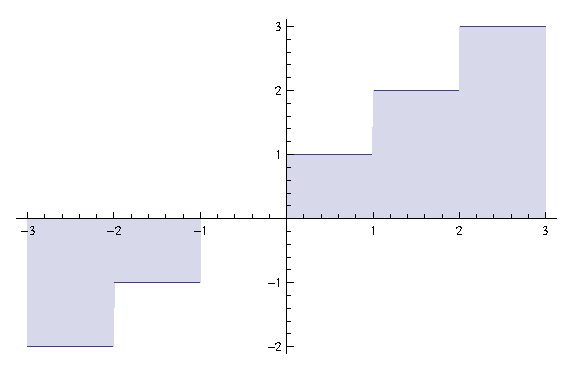
\includegraphics[width=\textwidth]{1.eps}
                \caption{i}
        \end{subfigure}%
        ~ %add desired spacing between images, e. g. ~, \quad, \qquad etc.
          %(or a blank line to force the subfigure onto a new line)
        \begin{subfigure}[b]{0.5\textwidth}
                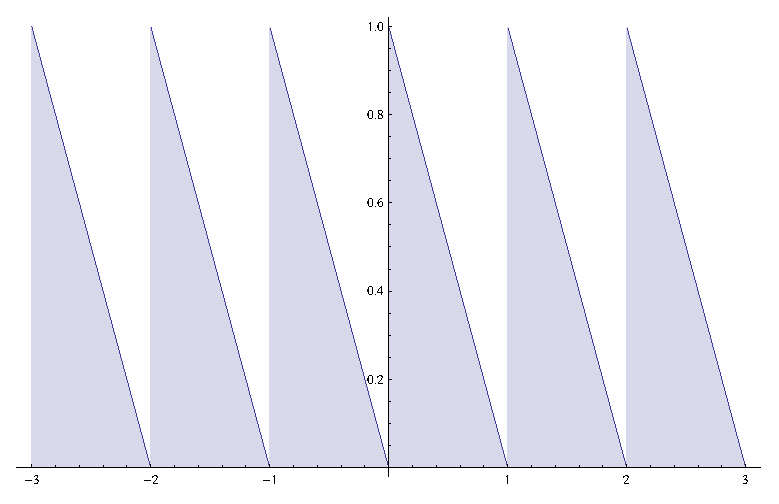
\includegraphics[width=\textwidth]{2.eps}
                \caption{ii}

 \end{subfigure}\\

        \begin{subfigure}[b]{0.5\textwidth}
                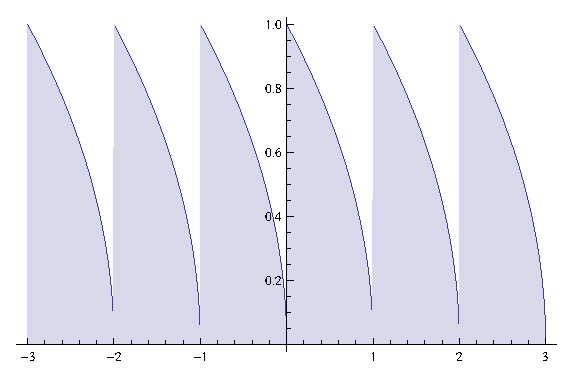
\includegraphics[width=\textwidth]{3.eps}
                \caption{iii}

        \end{subfigure}%
        \begin{subfigure}[b]{0.5\textwidth}
                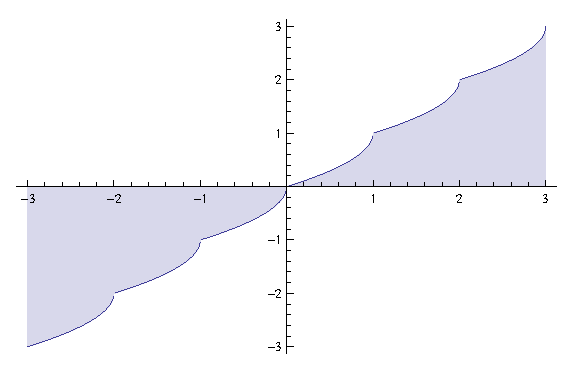
\includegraphics[width=\textwidth]{4.eps}
                \caption{iv}

           \end{subfigure}\\
                     \begin{subfigure}[b]{0.5\textwidth}
                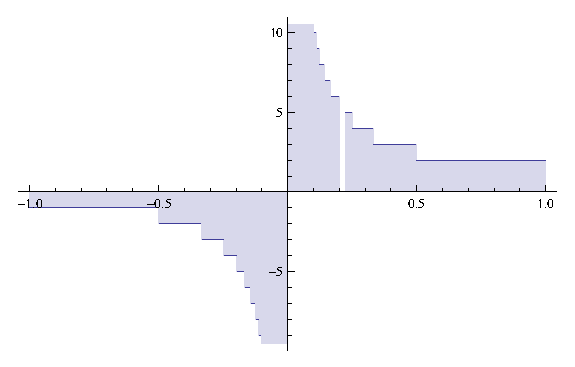
\includegraphics[width=\textwidth]{5.eps}
                \caption{v}

        \end{subfigure}%
        \begin{subfigure}[b]{0.5\textwidth}
                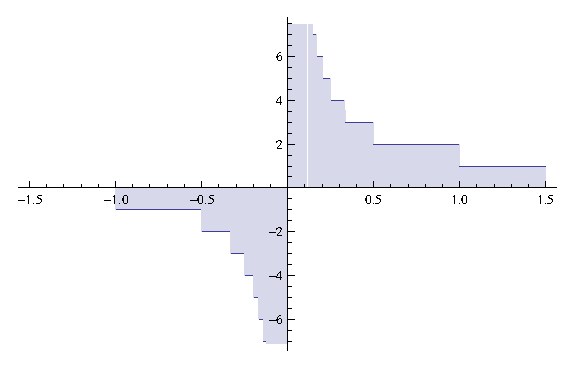
\includegraphics[width=\textwidth]{6.eps}
                \caption{vi}

               \end{subfigure}
\end{figure}
\end{document}